\documentclass[../main.tex]{subfiles}

\begin{document}
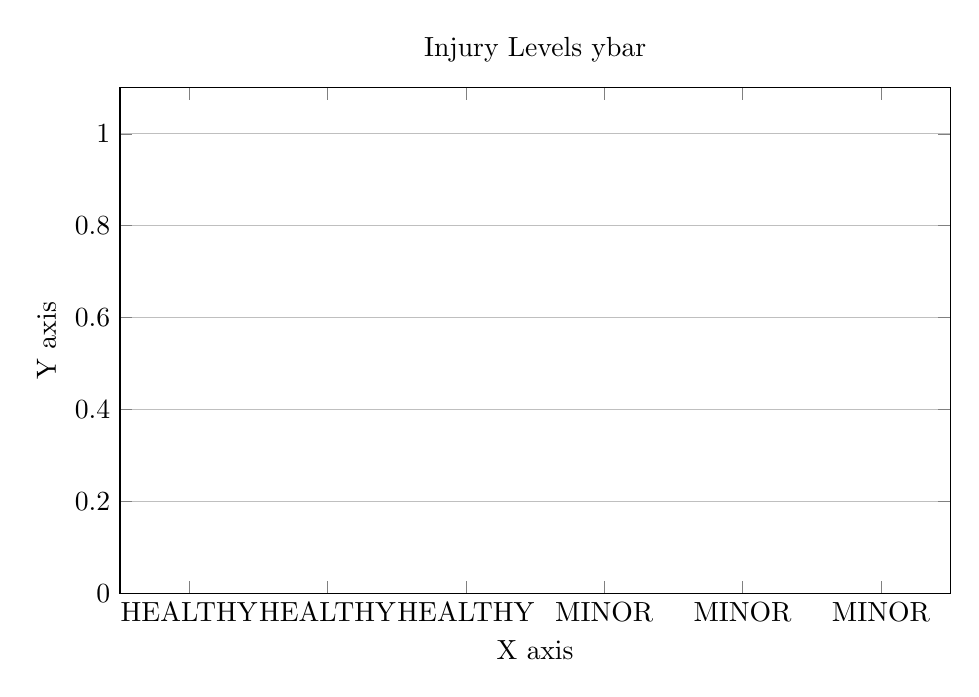
\begin{tikzpicture}
\begin{axis}[
title={Injury Levels}
ybar, % style of the histogram: clustered columns
width=\textwidth, % width of the plot
height=8cm, % height of the plot
xlabel={X axis}, % label for the x-axis
ylabel={Y axis}, % label for the y-axis
symbolic x coords={HEALTHY,MINOR,MODERATE,SERIOUS,	SEVERE,CRITICAL,FATAL}, % labels for the x-ticks
xtick=data, % position the x-ticks at the data points
ymin=0, % minimum value of the y-axis
legend style={at={(1,1)}, anchor=north east}, % position of the legend
legend cell align=left, % alignment of the legend cells
ymajorgrids=true, % display major grids
bar width=0.25cm % width of the bars
]
\addplot[color=teal] coordinates{}; % plot of the first histogram
\addplot[color=blue] coordinates{}; % plot of the second histogram
\addplot[color=cyan] coordinates{}; % plot of the third histogram
\addplot[color=violet] coordinates{}; % plot of the fifth histogram
\addplot[color=purple] coordinates{}; % plot of the first histogram
\addplot[color=magenta] coordinates{}; % plot of the second histogram
\legend{false \#1,  false \#2, false \#3, true \#1, true \#2, true \#3} % legend of the plot
\end{axis}
\end{tikzpicture}
\end{document}